\section{shell编程}

\begin{frame}{shell编程}
	\tableofcontents[currentsection]
\end{frame}

\subsection{shell 简介}
\begin{frame}{shell简介}
每一个操作系统都会有提供一个在命令行下用户和系统内核打交道的接口,一般我们称它为shell
\begin{itemize}
\item Windows Command Prompt(PowerShell)
\item sh 最原始的shell
	\begin{description}
	\item[bash] Bourne-Again Shell,来自sh的改进
	\item[ksh] Korn shell ,sh的超集
	\end{description}
\item csh C语言语法风格的shell
	\begin{description}
	\item[tcsh] csh的改进版本
	\end{description}
\item $\ldots$
\end{itemize}
\end{frame}

\begin{frame}{sh,bash 最广泛的脚本编程语言}
\begin{itemize}
\item shell = 命令执行的宏处理器
\item 直接调用Unix命令和内置的一些指令,在使用上,看不出区别
\item 完备的编程语言
\item 输入来源可以是:
	\begin{itemize}
	\item 来自终端
	\item 来自包含指令的文件
	\end{itemize}
\end{itemize}
\end{frame}

\subsection{bash 登录过程}

\begin{frame}[allowframebreaks]{bash登录过程}
\begin{itemize}
\item getty的程序负责等待用户登录,这就是我们在终端上看到的“login:”。 

\item  当用户输入用户名并回车后,getty进程将结束并启动login程序,即在终端显示字符串“password:”。

\item 接下来用户输入密码并回车,login将验证用户名密码是否与系统文件/etc/passwd中的记录以及/etc/shadow中的密码是否一致。 

\item 如果通过,则激活/etc/passwd中该用户记录行的最后一列的程序,如果没有设置,则启动/usr/bin/sh程序。

\item 这期间也将执行预定义好的用户环境脚本,这些初始化脚本执行结束后,终端将出现命令提示符等待用户输入命令,登录过程至此全部完成。 

\item 用户退出系统后,shell将退出,但系统会自动在该终端启动一个新的getty,等待用户登录。正如我们看到的好像“login:”永远不会消失一样。
\end{itemize}
\end{frame}

\subsection{bash如何执行启动脚本}

\begin{frame}[fragile,allowframebreaks]{bash如何执行它的启动文件}
\begin{block}{当bash是作为交互的登录 shell 启动的:}
\begin{verbatim} 
Login:root
Password:******
reading ~/.bash_login ... 
Last login: Thu May 26 10:26:56 2011 from 192.168.8.10
reading /etc/profile ... 
reading ~/.bashrc ... 
reading ~/.bash_profile ... 
[root@ ~]# 
\end{verbatim}
\end{block}

\begin{block}{以非交互式的 shell 指定 --login 选项启动的}
\begin{verbatim}
[root@ ~]# bash --login
reading /etc/profile ... 
reading ~/.bashrc ... 
reading ~/.bash_profile ... 
[root@ ~]# 
\end{verbatim}
\end{block}

\newpage

\begin{block}{以非交互式启动 shell }
\begin{verbatim}
[root@ ~]# bash
reading ~/.bashrc ... 
[root@ ~]# 
\end{verbatim}
\end{block}

\newpage

\begin{block}{如果 shell 是以与真实用户(组) id 不同的有效用户(组) id 来启动的, 并且没有 - 选项,那么它不会读取启动文件, 也不会从环境中继承 shell 函数. }
\begin{verbatim}
[root@ ~]# su 
reading ~/.bashrc ... 
[root@ ~]# su -
reading /etc/profile ... 
reading ~/.bashrc ... 
reading ~/.bash_profile ..
\end{verbatim}
\end{block}
\end{frame}

\begin{frame}{bash 保留字}
\begin{verbatim}
! case  do done elif else esac fi for function  
if in select then until while { } time [[ ]]
\end{verbatim}
\end{frame}

\subsection{bash 语法}

\begin{frame}[fragile,allowframebreaks]{bash 语法}
\begin{block}{Simple Commands}
\alert{Simple Commands 简单命令} 是一组词序列,第一个词定义为命令,它被成为第0个参数,其余词被作为这个命令的参数.
\end{block}

\newpage

\begin{block}{pipleline}
\alert{pipeline 管道} 是一组命令序列,用字符 | 分隔。管道的格式: 命令 command 的标准输出通过管道连接到命令 command2 的标准输入。连接是在命令指定的任何重定向之前进行的。

\begin{verbatim}
[root@ opt]# time ls -R |wc -l
50203

real    0m2.309s
user    0m0.178s
sys     0m0.341s
[root@ opt]#
\end{verbatim}
\end{block}

\begin{block}{命令序列}
\alert{序列} 序列是一个或多个管道,用操作符 ;, \&,\&\&, │, 或 <newline>新行符结束\begin{description}
\item[cmd1; cmd2; $\cdots$] 顺序执行
\item[cmd1 \&] 异步执行
\item[cmd1; \&\& cmd2 $\cdots$] 前一个命令执行成功才会执行后一个命令
\item[cmd1 || cmd2 ] cmd1返回非0值才会执行cmd2
\end{description}
\end{block}
\end{frame}


\begin{frame}[fragile,allowframebreaks]{复合命令}
\begin{block}{(command; command $\cdots$)}
( $ \cdots $ )将在一个子 shell 中执行。变量赋值和影响 shell 环境变量的内建命令在命令结束后不会再起作用。返回值是序列的返回值 \\
(ls) ;  (ls)
\end{block}

\newpage

\begin{block}{\{ commands; \} }
序列将在当前 shell 环境中执行。序列必须以一个新行符或分号结束。注意与元字符 ( 和 )不同, \{ 和 \} 是 reserved words(保留字),必须出现在能够识别保留字的场合。由于它们不会产生断词,它们和序列之间必须用空格分开。
\begin{verbatim}
#{ ls; }              //  wrong:  {ls}  {ls;}
#{ ls; } ; { df; }
\end{verbatim}
\end{block}

\newpage

\begin{block}{(( expression )) }
表 达 式 expression 赋值语句。如果表达式的值非零,返回值就是  0 ;否则返回值是 1。这种做法和 let “expression” 等价。
\begin{verbatim}
[root@ ~]# w=3; y=4; ((z=w+y)) ; echo $z
7
[root@ ~]# w=3; y=4; let z=w+y ; echo $z
7
\end{verbatim}
\end{block}

\newpage

\begin{block}{[[ expression ]] }
返回 0 或 1,取决于条件表达式 expression 求值的情况。表达式的原语组成稍后介绍;
\begin{verbatim}
[root@ ~]# [[ 3 != 3 ]] ; echo $?
1
[root@ ~]#  a="wer";[ $a = wer ]; echo $?
0
[root@ ~]# ((23>34)); echo $?
1
\end{verbatim}
\end{block}
\end{frame}

\subsection{bash 语句}

\begin{frame}[fragile,allowframebreaks,plain]{bash 语句}

\begin{block}{for name [ in word ] ; do list; done }
in 之后的一系列词会被扩展,产生一个项目列表。变量 name 被依次赋以这个列表中的每个元素,序列 list 每次都被执行。返回值是最后一个命令的返回值。
\begin{verbatim}
[root@~]# for i in a b c d;do echo $i; done
a
b
c
d
\end{verbatim}
\end{block}

\newpage

\begin{block}{for (( expr1; expr2; expr3 )); do list; done }
\begin{verbatim}
[root@~]# for (( i=0; i<10;i++ )); echo $i; done
0
1
2
3
...
8
9
\end{verbatim}
\end{block}

\newpage

\begin{block}{select name [ in word ]; do list; done}
\begin{verbatim}
#!/bin/bash
word="a b c"
select i in $word; do
	case $i in 
		a) echo "I am A"
		;;
		*) break
		;;
esac	
done
\end{verbatim}
\end{block}

\newpage

\begin{block}{执行结果}
\begin{verbatim}
[root@~]#./test.sh
./test.sh
1) a
2) b
3) c
#? 1
I am A
#? 2
\end{verbatim}
\end{block}

\newpage

\begin{block}{if条件语句}
\begin{verbatim}
if list; then
    list;
    [elif list; then list;]
    ...
    [else list; ]
fi
\end{verbatim}
\end{block}

\newpage

\begin{block}{loop \& function}
\begin{verbatim}
while list; do list; done
until list; do list; done
[ function ] name () {list;} 
name [ arg1,arg2,...]
\end{verbatim}
\end{block}
\end{frame}


\begin{frame}{特殊参数}
\begin{description}
\item [\$*] \$* 扩展为位置参数, “\$*” 等价于 “\$1c\$2c $\ldots$”, 这里 c 是变量 IFS 的第一个字符。如果没有设置 IFS,用空格分隔。
\item[\$@ ]等价于 "\$1" "\$2" $\ldots$
\item [\$\#] 扩展为位置参数的个数,以十进制表示。
\item [\$? ] 扩展为最近执行的前台管道的状态。
\item [\$\$] 扩展 为shell 的进程 ID。
\item [\$!] 扩展为最近一次执行的后台 (异步) 命令的进程号。
\item [\$0 ] 启动脚本名,或者指向通过bash -c 运行的第一个参数
\item [\$\_]  shell 启动时,设置为 shell 或参数中被执行的 shell 脚本的绝对路径名。
\end{description}
\end{frame}

\begin{frame}[allowframebreaks]{常用的shell变量}
\begin{description}
\item [HOSTNAME] 自动设置为当前的主机名
\item [OLDPWD] 上一次命令 cd 设置的工作目录
\item [HOSTTYPE] 标识当前脚本运行的机器类型 "x86\_64"
\item [PPID]  当前进程的父进程号,只读变量
\item [PWD]  当前工作目录
\item [SECONDS] 返回当前脚本自运行以来的秒数。如果向 SECONDS赋 值,此后对它的引用将返回自赋值时起的秒数加上所赋予的值。
\item [RANDOM] 每次引用这个参数,都会产生 0 到 32767 之间的随机整数
\item [UID] 当前用户的 ID,在启动时初始化。这个变量是只读的
\item [LANG] 用来决定没有特意用LC\_变量制定的语言环境项
\item [LC\_ALL] 这个变量超与了LANG和所有其他制定语言环境项的LC\_变量
\item [PATH] 搜索命令的路径,路径之间用冒号(:) 分隔
\item [TMOUT] 如果设置为大于 0 的值,TMOUT 被当作内建命令 read 的默认超时等待时间。如果等待终端输入时, TMOUT 秒之后仍然没有输入,bash 将退出.
\item [HISTFILE] 保存命令历史的文件名。默 认 值 \textasciitilde{}/.bash\_history 如果取消定义,在交互式 shell 退出时命令历史将不会保存
\item [HISTSIZE] 命令历史中保存的历史数量
\item [HOME] 当前用户的个人目录;内建命令 cd 的默认参数。波浪线扩展为此变量
\item [HOSTFILE] 包含一个格式和 /etc/hosts 相同的文件名。当 shell 需要补全主机名时要读取它
\end{description}
\end{frame}

\begin{frame}{Arrays 变量}
Bash  提供了一维数组变量。任何变量都可以作为一个数组 \\
要显式地 定义 一 个 数 组 ,使用 declare -a name。数组的大小没有上限,从 0 开始\\
如果变量赋值时使用语法 name[n]=value,会自动创建数组。\\
数组的任何元素都可以用 \$\{name[subscript]\} 来引用。花括号是必须的,以避免和路径扩展冲突。\\
如果 subscript 是 @ 或是 *,它扩展为 name 的所有成员。\\
这两种下标只有在双引号中才不同。在双引号中,\$\{name[*]\} 扩展为一个 词, 由所有数组成员的值组成,用特殊变量 IFS 的第一个字符分隔;\$\{name[@]\}将 name 的每个成员扩展为一个词
\end{frame}

\begin{frame}{命令行扩展}
Bash有 七 种 类 型的扩展:
\begin{enumerate}
\item brace expansion( 花 括 号 扩 展)
\item  tilde expansion(波浪线扩展)
\item parameter and variable expansion(参数和变量扩展)
\item command substitution(命令替换)
\item arithmetic  expansion(算术扩展)
\item  word splitting(词的拆分)
\item pathname expansion(路径扩展)
\end{enumerate}
例如, a\{d,c,b\}e 扩展为 ‘ade ace abe’。这种结构通常用来简写字符串的公共前缀较长的情况,例如 \\
mkdir /usr/local/src/bash/\{old,new,dist,bugs\} \\
chown root /usr/\{ucb/\{ex,edit\},lib/\{ex?.?*,how\_ex\}\}
\end{frame}

\begin{frame}{模式匹配}
\begin{description}
\item [ * ] 匹配任何字符串包括空串
\item [ ? ] 匹配任何一个字符
\item [ $\cdots$] 匹配所包含的任何字符之一 
\item [ - ] 范围表达式,任何排在他们之间的字符,都会被匹配
\end{description}
\end{frame}

%\begin{frame}{重定向}
%bash允许使用下面的几种结构将标准输入和标准错误输出重定向到用户定义的字符流中
%\begin{itemize}
%\item \&>word
%\item >\&word
%\item >word \&
%\item >word 2>\&1
%\end{itemize}
%\end{frame}

\begin{frame}[fragile]{Here Documents}
这种重定向使得shell从当前源文件中读取输入,知道遇到仅包含关键字的一行为止
\begin{verbatim}
#!/bin/sh
cat << EOF
     hello
    this is 
    here 
    documents
EOF 
\end{verbatim}
\href{http://blog.wgzhao.com/2009/08/24/here-documents-in-bash.html}{几种特别的用法}
\end{frame}

\begin{frame}[allowframebreaks]{条件表达式}
条件表达式用于 [[ ]]复合命令以及内建命令 test 和 [ ]中,用来测试文件属 性,进行字符串和算术比较
\begin{description}
\item [-a file] 如果 file 存在则为真
\item [-b file] 如果 file 存在且为块设备则为真
\item [-c file] 如果 file 存在且为字符设备则为真
\item [-d file] 如果 file 存在且是一个目录则为真
\item [-e file] 如果 file 存在则为真
\item [-f file] 如果 file 存在且为普通文件则为真
\item [-g file] 如果 file 存在且是设置组ID的 (sgid) 则为真
\item [-h file]  file 存在且为符号链接则为真
\item [-k file] 如果 file 存在且设置了 ‘‘sticky’’ 位 (粘滞位) 则为真
\item [-p file] 如果 file 存在且是一个命名管道 (FIFO) 则为真
\item [-r file] 如果 file 存在且可读则为真
\item [-s file] 如果 file 存在且大小大于零则为真
\item [-t fd] 如果文件描述符 fd 是打开的且对应一个终端则为真
\item [-u file] 如果 file 存在且是设置用户ID的 (suid) 则为真
\item [-w file]		如果 file 存在且可写则为真
\item [-x file]		如果 file 存在且可执行则为真
\item [-O file]		如果 file 存在且为有效用户ID所拥有则为真
\item [-G file]		如果 file 存在且为有效组ID所拥有则为真
\item [-L file]		如果 file 存在且为符号链接则为真
\item [-S file]		如果 file 存在且为套接字则为真
\item [-N file]		如果 file 存在且上次读取后被修改过则为真
\item [-z string] 如果string的长度为0 则为真
\item [-n string] 如果string的长度非0则为真

\item [file1 -nt file2] 如果 file1 比 file2 要新 (根据修改日期)则为真
\item [file1 -ot file2] 如果 file1 比 file2 更旧则为真
\item [file1 -ef file2]	如果 file1 和 file2 指的是相同得inode号则为真
\item [string1 == string2] 如果字符串相等则为真, = 可以用于使用==的场合来兼容POSIX规范
\item [string1 != string2] 如果字符串不相等则为真
\item [string1 < string2] 如果string1 在当前语言环境的字典顺序中排在string2之前则为真
\item [string1 > string2] 如果string1 在当前语言环境的字典顺序中排在string2之后则为真
\item [arg1 \underline{OP} arg2 ] OP 是 -eq, -ne, -lt, -le, -gt,-ge之一,这写算术操作返回真,如果arg1与args2分别是相等,不等,小于等于,大于,大于等于关系.arg1和arg2可以是正负整数.
\end{description}

\end{frame}

\subsection{grep}

\begin{frame}{grep}
grep (global search regular expression and print out the line)是一种强大的文本搜索工具,它能查找文件中指定的正则表达式,并打印含有该表达式的所有行。\\
使用grep的好处在于,不需要启动vi、ex等编辑器来执行查找,由于是命令行,又可以进行文件批量扫描查找,并且不需要将将正则表达式包含到斜线中
\end{frame}

\begin{frame}{grep常用参数}
\begin{description}
\item [-c ] 只输出匹配行的计数
\item [ -i ] 不分区大小写(只适用于单字符)
\item [ -l ] 只输出包含匹配字符的文件名
\item [ -n ] 显示匹配行及行号
\item [ -v ] 显示不包含匹配文本的所有行
\end{description}
\href{http://wangcong.org/blog/?p=1439}{http://wangcong.org/blog/?p=1439}
\end{frame}


\subsection{sed}

\begin{frame}[fragile,allowframebreaks]{sed}

\begin{block}{\alert{d} 删除命令}
\begin{itemize}
\item sed -e '1d' /etc/profile
\item sed -e '/\^\#/d' /etc/profile
\item sed -e '1,5d' /etc/profile
\end{itemize}
\end{block}

\begin{block}{\alert{s} 替换命令}
\begin{itemize}
\item sed 's/apple/orange/g' file
\item sed -n 's/\(new\) day/\textbackslash{}1 year/p' file 
\end{itemize}
\end{block}

\begin{block}{\alert{,} 行范围指定符}
\begin{itemize}
\item sed '/ifndef/,/endif/s/\$/END/' file \\
修改从ifndef到endif之间的所有行,并将各行末尾加上字符串END 
\item sed -e '/\#ifndef/,/\textbackslash{}\#endif/s/aaa/bbb/' prog.h
\end{itemize}
\end{block}

\begin{block}{\alert{a\textbackslash} 追加命令}
a\textbackslash 表示追加文本。注意a命令要以“\textbackslash{}” 结尾,追加内容将被加入匹配行的下一行 \\
\verb| sed '/^##/a\ this is an appended line ' file |

本例所做的操作是把所有以“\#\#”开头的行后面附加一行文本
\end{block}

\begin{block}{\alert{i\textbackslash}  插入命令}
i命令和a命令一样要以“\textbackslash" 结尾, 所不同的是, 它所追加的内容将被插入匹配行的前一行 \\
sed ‘/\^\#\# /i\textbackslash{} This is an inserted line’ file \\
本例所做的操作是把所有以“\#\#”加空格开头的行前面插入一行文本
\end{block}

\begin{block}{\alert{n} 下一行命令}
这个命令也很常用,很多系统配置文件的修改操作可以看到它。\\
sed '/Section \textbackslash{}"Device\textbackslash"{}/\{n;n;s/i810/vesa/;\}’ file \\
本例所做的操作是先找到以Section “Device”开始的行,找到后,对它的下面第二行中的i810替换为vesa
\end{block}

\begin{block}{sed单行脚本快速参考}

\href{http://sed.sourceforge.net/sed1line\_zh-CN.html}{http://sed.sourceforge.net/sed1line\_zh-CN.html}
\end{block}
\end{frame}

\subsection{awk}

\begin{frame}{awk}
\alert{awk} = \alert{A}ho \alert{W}einberger \alert{K}ernighan
\begin{quote}
Awk is a programming language designed to make many common information  retrieval  and text manipulation tasks  easy to state and to perform.
\end{quote}
\end{frame}

\begin{frame}{awk版本}
\begin{description}
\item[awk] Bell实验室的原始版本(Verion 7 UNIX, \textbackslash{} 1978) + 最新的POSIX awk 版本
\item[nawk] New awk,大约1989年随SVR4发布的版本
\item[gawk] awk的GNU组织实现版本,大部分Linux发行版本都有他.
\item[mawk] Michael的版本
\item[$\cdots$]
\end{description}
除了一些细微差别外,所有的这些发行版本功能基本相当.
\end{frame}

\begin{frame}{基本概念}
\begin{itemize}
\item awk 从文件或者标准输入读取,然后输出到标准输出
\item awk 识别 文件(file) , 记录(record) 和域(field)的概念
\item 文件有记录组成,缺省情况下,文件的每一行称为一条记录
\item awk 同一时刻只操作一条记录
\item 记录有一个或多个域组成,缺省情况下,域之间由空格或者制表符分隔(数目不限)
\item awk通过\${}1 访问第一个域,通过\${}2 访问第二个域,以此类推
\item 
\end{itemize}
\end{frame}

\begin{frame}{awk的基本结构}
\begin{itemize}
\item 一个awk语句或者脚本是下列语句的组合 \\
\alert{pattern}   \{ action \} \\
\alert{pattern}   \{ action \} \\
$\cdots$

\item \alert{pattern} 做为 action之否执行的一个判断
\item patterns 可以是:
	\begin{itemize}
		\item 正规表达式(regular expressions)
		\item 算术相关表达式
		\item 字符串值表达式
		\item 任意布尔值的组合
	\end{itemize}
\end{itemize}
\end{frame}

\begin{frame}[fragile]{一个简单的例子}
\begin{exampleblock}{需求}
从 \textbf{/etc/passwd} 文件获取用户 \textbf{wgzhao} 的用户ID号 \\
假设 /etc/passwd 文件由下面几行组成: \\
\begin{verbatim}
arun:x:504:504::/home/arun:/bin/bash
wgzhao:x:500:500::/home/wgzhao:/bin/bash
hacluster:x:501:501::/home/optima:/bin/bash
nfsbody:x:13:7::/var/lib:/sbin/nologin
\end{verbatim}

awk读取/etc/passwd文件,会认为:  \\
一行就是一个记录,因此这里共有4条记录 \\
一个记录由7个域组成,分隔符为":" (不是缺省分隔符)
\end{exampleblock}
\end{frame}

\begin{frame}{一个答案}
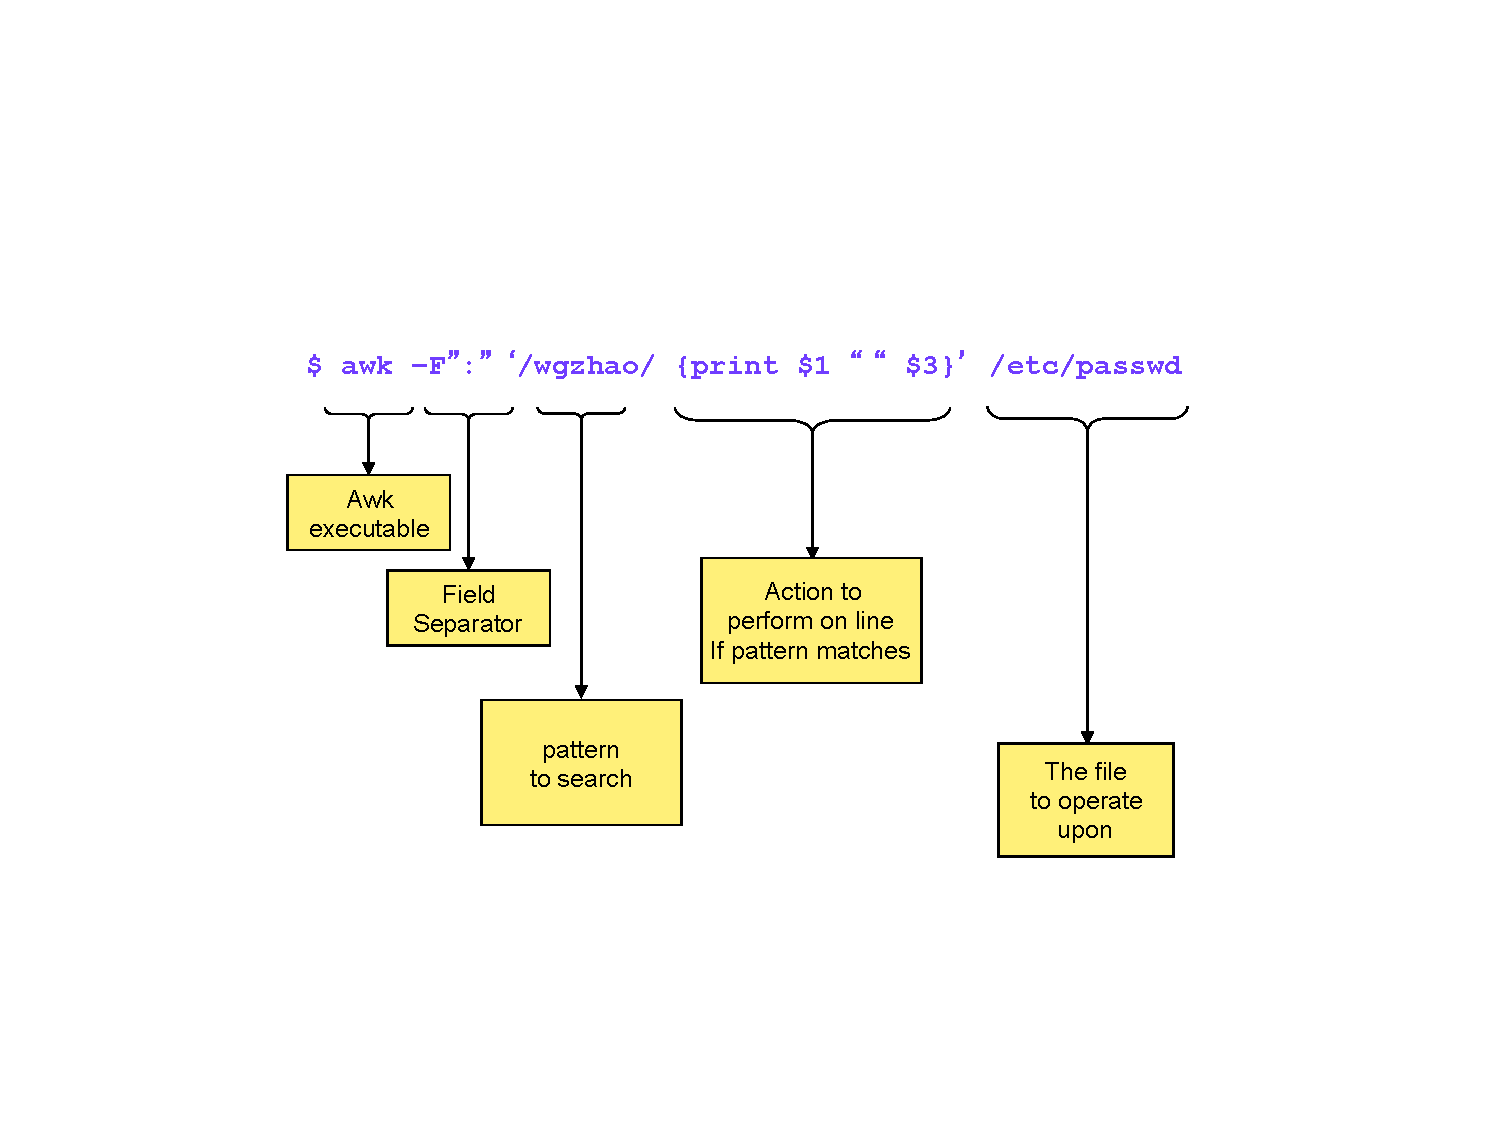
\includegraphics[scale=.6]{awk-example}
\end{frame}

\begin{frame}[fragile]{执行结果}
\begin{verbatim}
[root@~]# awk -F":" ‘/wgzhao/ {print $1 " " $3}’ /etc/passwd 
 wgzhao 500
\end{verbatim}

换一个写法
\begin{verbatim}
[root@ ~ ]# awk ‘BEGIN { FS=“:” } /arun/ {print $1 " " $3}’ /etc/passwd 
 wgzhao 500
\end{verbatim}
\end{frame}

\begin{frame}[fragile,allowframebreaks]{运行awk程序}
一般来说,我们有四种方式来运行awk程序
\begin{enumerate}
\item 单行脚本模式 \\
  e.g  awk 'program' input-file1 input-file2  $\cdots$
\item 没有输入文件,直接从终端读取 \\
\begin{verbatim}
$ awk 'program' <ENTER>
<input lines>
<input lines>
...
ctrl-d
\end{verbatim}
\item 将awk代码写入脚本,然后调用 \\
e.g  awk -f source-file input-file1 input-file2 $\cdots$

\item 制作成可执行脚本,类似shell脚本
\begin{verbatim}
#!/bin/awk -f 
# a simple awk program
/foo/ { print $1 }
\end{verbatim}
chmod +x hello \\
./hello file.txt
\end{enumerate}
\end{frame}

\begin{frame}[fragile,allowframebreaks]{高级awk特性}
\begin{itemize}
\item Awk 从C语言里借鉴了很多
\item if 循环, for 循环 和while 循环和C语言的结构相同
\item Awk的变量在内部当作字符串存储 \\
\begin{verbatim}
x = "1.01"
x = x + 1
print x
\end{verbatim}
\item awk 里的比较操作符有: "==","<",">","<=",">=","!=","~","!~"

\item "~" 表示匹配(matches),"!~"则表示不匹配

\item awk 里的算术操作符有: "+","-","/","*"
\item "\^" 是乘方运算 , "\%" 是模运算
\item 所有 C 操作符,比如"++","--","+=","-=","/=" 等在awk里也有效
\item awk 支持一维数组,可以存储字符串或数值
\end{itemize}
\end{frame}

\begin{frame}[fragile,allowframebreaks]{awk 实例}
\begin{block}{打印/etc/passwd的所有行}
\begin{verbatim}
$ awk '{ print $0 }' /etc/passwd
\end{verbatim}
\end{block}

\begin{block}{打印/etc/passwd所有行的第一列和第三列,分隔符为":"}
\begin{verbatim}
awk -F":" '{ print "username: " $1 "\t\tuid:" $3" }' /etc/passwd 
\end{verbatim}
\end{block}

\begin{block}{计算/etc/passwd文件里空白行数}
\begin{verbatim}
$ awk –f script1.awk /etc/passwd
  script1.awk
  BEGIN{ x=0 }# The BEGIN block is executed before processing the file
  /^$/ { x=x+1 } # For every null line increment the count
  END { print "I found " x " blank lines. :)" } #Executed at the end
\end{verbatim}
\end{block}

\begin{block}{修改记录分隔符的例子}
\begin{verbatim}
awk 'BEGIN { RS = "/" } ; { print $0 }' file1.txt
\end{verbatim}
RS = Record Separator ,缺省是"\textbackslash{}n",上述例子表示把记录分隔符修成"/",因此awk按照"/"符号来对file1.txt区分断行
\end{block}
\end{frame}
